\documentclass[tikz,border=8pt]{standalone}

\usepackage{pgfplots}
\pgfplotsset{compat=1.18}
\usepackage{xcolor}

% ---- 11 种高饱和、鲜亮配色 ----
\definecolor{barA}{HTML}{1A6FDF} % 亮蓝
\definecolor{barB}{HTML}{27C93F} % 鲜绿
\definecolor{barC}{HTML}{FF3B30} % 醒目红
\definecolor{barD}{HTML}{8E44FF} % 电光紫
\definecolor{barE}{HTML}{FF9500} % 明橙
\definecolor{barF}{HTML}{00C2D1} % 亮青
\definecolor{barG}{HTML}{E5177B} % 玫红
\definecolor{barH}{HTML}{FFD500} % 亮黄
\definecolor{barI}{HTML}{00A878} % 翡翠绿
\definecolor{barJ}{HTML}{7B4DFF} % 靛紫
\definecolor{barK}{HTML}{FF6B00} % 焦橙

\begin{document}

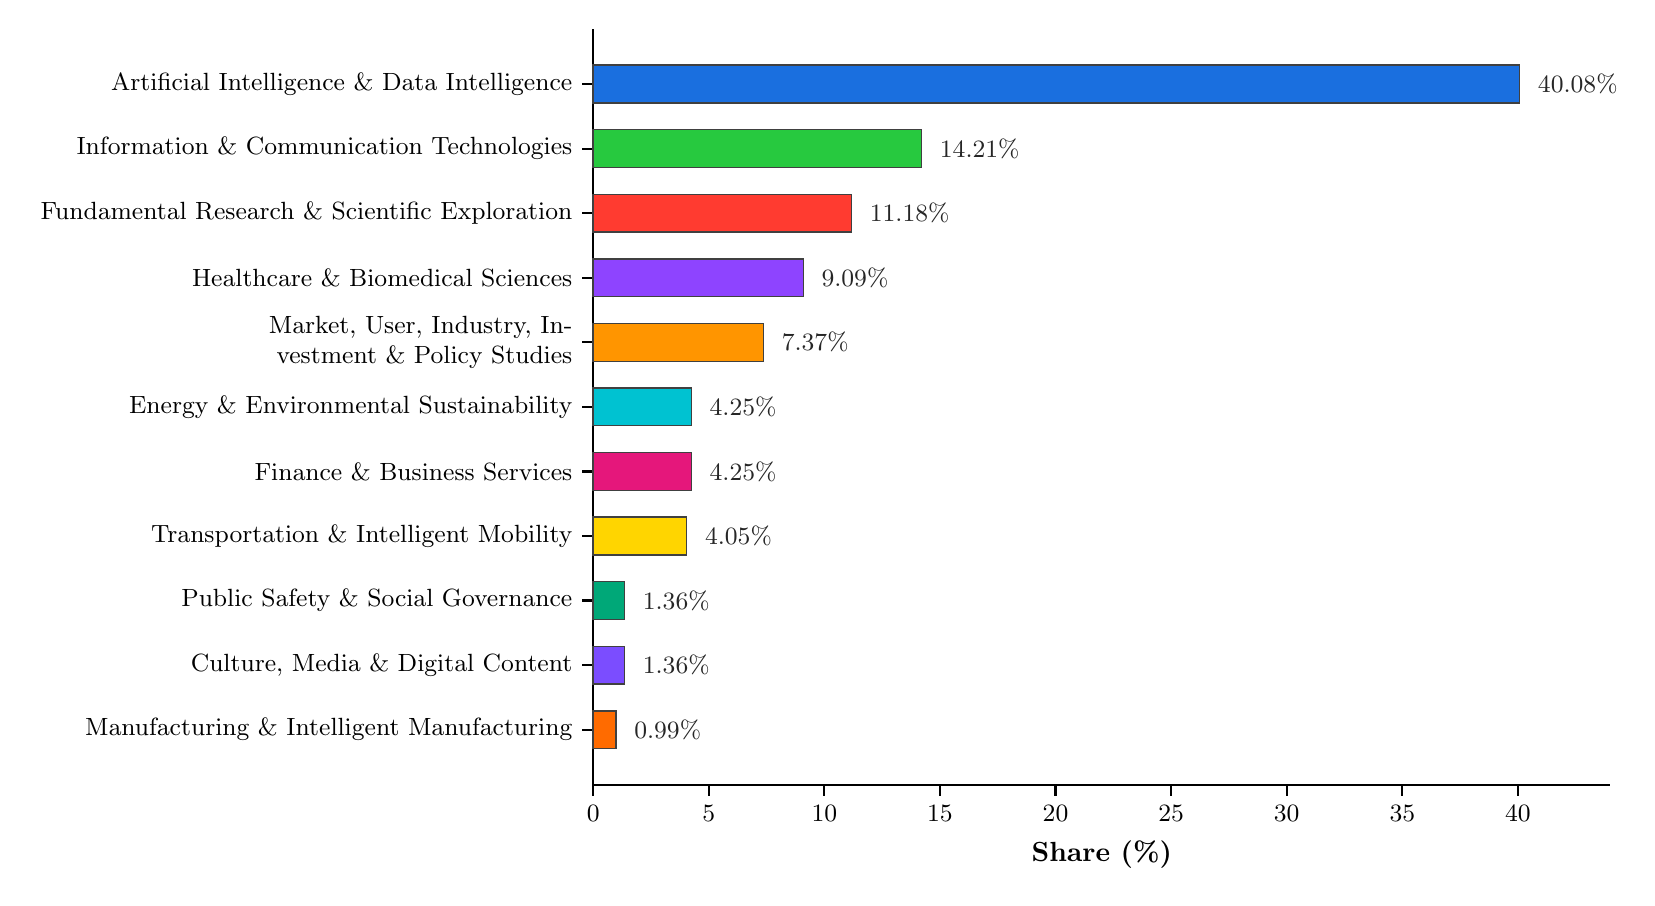
\begin{tikzpicture}
    \begin{axis}[
        width=14.5cm,
        height=12.5cm,
        xmin=0, xmax=44,
        y=0.82cm,                    % 每个类目行的间距
        xbar,                        % ---- 横向柱状图 ----
        bar width=0.48cm,
        axis lines=left,             % 只保留左、下轴
        axis line style={-, black, line width=0.9pt},
        xlabel={Share (\%)},
        xlabel style={font=\normalsize\bfseries},
        xtick={0,5,10,15,20,25,30,35,40},
        xticklabel style={font=\small},
        yticklabel style={
            font=\small,
            text width=6.8cm,
            align=right
        },
        tick align=outside,
        tick style={black, line width=0.8pt},
        major tick length=4pt,
        enlarge y limits={abs=0.7cm},
        clip=false,
        ytick={1,2,3,4,5,6,7,8,9,10,11},
        yticklabels={
            {Manufacturing \& Intelligent Manufacturing},
            {Culture, Media \& Digital Content},
            {Public Safety \& Social Governance},
            {Transportation \& Intelligent Mobility},
            {Finance \& Business Services},
            {Energy \& Environmental Sustainability},
            {Market, User, Industry, Investment \& Policy Studies},
            {Healthcare \& Biomedical Sciences},
            {Fundamental Research \& Scientific Exploration},
            {Information \& Communication Technologies},
            {Artificial Intelligence \& Data Intelligence},
        },
        nodes near coords style={
            font=\small,
            anchor=west,
            xshift=3pt,
            text=black!85,
        },
        bar shift=0pt,
        cycle list={},
    ]
    % ---- 每根柱子独立上色；y 坐标 1=最底，11=最顶 ----
    \addplot[xbar, fill=barK, draw=black!75, line width=0.5pt,
        nodes near coords={0.99\%}]  coordinates {( 0.99,1)};
    \addplot[xbar, fill=barJ, draw=black!75, line width=0.5pt,
        nodes near coords={1.36\%}]  coordinates {( 1.36,2)};
    \addplot[xbar, fill=barI, draw=black!75, line width=0.5pt,
        nodes near coords={1.36\%}]  coordinates {( 1.36,3)};
    \addplot[xbar, fill=barH, draw=black!75, line width=0.5pt,
        nodes near coords={4.05\%}]  coordinates {( 4.05,4)};
    \addplot[xbar, fill=barG, draw=black!75, line width=0.5pt,
        nodes near coords={4.25\%}]  coordinates {( 4.25,5)};
    \addplot[xbar, fill=barF, draw=black!75, line width=0.5pt,
        nodes near coords={4.25\%}]  coordinates {( 4.25,6)};
    \addplot[xbar, fill=barE, draw=black!75, line width=0.5pt,
        nodes near coords={7.37\%}]  coordinates {( 7.37,7)};
    \addplot[xbar, fill=barD, draw=black!75, line width=0.5pt,
        nodes near coords={9.09\%}]  coordinates {( 9.09,8)};
    \addplot[xbar, fill=barC, draw=black!75, line width=0.5pt,
        nodes near coords={11.18\%}] coordinates {(11.18,9)};
    \addplot[xbar, fill=barB, draw=black!75, line width=0.5pt,
        nodes near coords={14.21\%}] coordinates {(14.21,10)};
    \addplot[xbar, fill=barA, draw=black!75, line width=0.5pt,
        nodes near coords={40.08\%}] coordinates {(40.08,11)};
    \end{axis}
\end{tikzpicture}

\end{document}
